\section{Introduction}

Since its discovery, the Dunhuang Grottoes have been an important site for the study of Buddhist art and
several important aspects of Chinese history, including the trade events via the Silk Road, etc.
While a large quantity of artefacts like the murals and sculptures have survived thousands of years
to be presented in this modern age, the artefacts are facing significant threats from various factors.
A study of \apaciteassub{Jiang2023-Weather-Dunhuang} has shown that the despite the lack of immediate risk
of preservation due to the drastic climate change in the past few decades, the artefacts are still
prone to deterioration due to the weathering effects of the natural environment. Therefore, the
preservation of the Dunhuang treasures is of utmost importance and a race against time
(\apaciteaspar{Yu2022-AI-Dunhuang}). Measures with high efficiency are needed to ensure the survival
of the cultural heritage.

In view of the above, the Dunhuang Research Academy (DHA) was established in 1944 and is now devoted to
applying modern technologies to the preservation of the Dunhuang Grottoes. While one takes advantage of
the efficiency and convenience of modern technologies, such as Artificial Intelligence (AI), one must
also be careful about the potential damages that may be imposed on the cultural heritage.
This essay aims to explore the current applications of the AI technology in the preservation of the 
Buddhist heritage, using the Dunhuang Caves as a case study. In the Literature Review section, some
cutting-edge AI applications in the archaeological field will be briefly explored. Then, in the
following two sections, the benefits and potential risks of these applications will be discussed.
Finally, a conclusion on the topic will be included, with a hope that the discussion would provide new
insights into the process of critically evaluating the use of AI in the preservation of cultural heritage.

\subsection{Terminology}

Since the topics ``cultural heritage'', ``preservation'' and ``AI'' are all broad, it may be helpful if
these terms are defined before the discussion commences. 

\subsubsection{Buddhist Heritage and Cultural Heritage}

In the context and the scope of discussion of this essay, the term ``Buddhist heritage'' and ``cultural
heritage'' are treated as the same, and they refer to both the artefacts and sites of the Dunhuang Grottoes.
The ``artefacts'' include the mural paintings, sculptures, manuscripts that were recovered from the Library
Cave (Cave 17) and other caves. The ``sites'' refer to the region, and the caves' architectural and structural
designs and features. This definition is consistent with that of the current standard as suggested by
\apaciteassub{UNESCO2024-Cultural-Heritage}.

\subsubsection{Preservation}

As suggested by \apaciteassub{UNESCO2024-Conservation}, the conservation and preservation of cultural heritage
are means taken to elongate the lifespan of the heritage and to convey its significance to the future
generations. Therefore, the term ``preservation'' would imply two aspects: the technical aspect of 
protecting the existence of the artefacts and sites, and the human aspect of public education and raising
awareness.

\subsubsection{Artificial Intelligence}

Contrary to the common generic definition of AI as ``the simple theory of human intelligence being
exhibited by machines'' (\apaciteaspar{Helm2020-AI-Orthopedics}, p. 69), this essay will refer to AI simply
as a set of tools utilising Machine Learning (ML), Convolutional Neural Networks (CNNs), Large
Language Models (LLMs), and Natural Language Processing (NLP) technologies
dedicated to the analysis and processing of images and texts for the purpose of
preserving cultural heritage.

\section{Literature Review}

Current AI applications in the study and preservation of Dunhuang Grottoes can be roughly categorised into
image-related techniques and text-related techniques.

\subsection{Computer Vision and Image Processing}

Algorithms specialised in computer vision and image processing, such as CNNs, Revolutional Neural Networks
(RNNs), and Generative Adversarial Networks (GANs), and hybrids of these algorithms are most prominently
used in the handling the murals of the Dunhuang Grottoes (\apaciteaspar{Fu2025-AI-Intangible-Cultural-Heritage};
\apaciteaspar{Yu2022-AI-Dunhuang}).

For the restoration of damaged murals, conventional patch-based methods
(\apasecciteaspar{Ballester et al.}{2001}{Yu2022-AI-Dunhuang}; \apasecciteaspar{Bertalmio}{2000}{Yu2022-AI-Dunhuang})
allowed automatic inpainting of small and simple damaged areas. Their inability to handle larger and more complex
missing areas have been overcome by modern use of CNNs (\apasecciteaspar{Pathak et al.}{2016}{Yu2022-AI-Dunhuang};
\apasecciteaspar{Yang et al.}{2017}{Yu2022-AI-Dunhuang}).
In recent years, \apasecciteassub{Song et al.}{2018}{Yu2022-AI-Dunhuang} proposed a more modern approach,
allowing the restoration and inpainting be context-aware, i.e. the algorithm would reconstruct the missing parts
by considering the surrounding context, rather than simply predicting pixels mathematically.
Similar means include systems built on CNNs and the ResNet-50 architecture, which are employed by the British
Museum and Le Musée du Louvre (the Louvre Museum) for damage recognition
(\apaciteaspar{Fu2025-AI-Intangible-Cultural-Heritage}).
Recent studies carried out by \apaciteassub{Chen2024-Mural-Inpainting} proposed a hybrid approach of joint
learning, further improving the errors produced by the AI models by allowing the models to learn from the global
context of the murals, rather than just the local context.

For creating arts in the visual style of the Dunhuang murals through AI, specialised algorithms referred to as
the ``style transfer'' algorithms are used (\apaciteaspar{Sun2023-Dunhuang-Patterns};
\apaciteaspar{Yu2022-AI-Dunhuang}). While \apaciteassub{Yu2022-AI-Dunhuang} mentioned certain limitations of the
algorithms built on the CNNs, such as lack of flexibility and optimisation, an experiment carried out by 
\apaciteaspar{Sun2023-Dunhuang-Patterns}, as shown in Figure \ref{fig:style-transfer-showcase}
displayed satisfactory results in transferring
the visual styles of the Dunhuang murals from different dynasties onto modern images.
Apart from application on Dunhuang murals,
a recent study by \apaciteassub{Zhang2023-AI-New-Year-Prints} also mentioned advanced techniques for generating
cultural and creative products by replicating visual styles from the input.

\begin{figure}
    \caption{Examples of results of merging Dunhuang art styles with modern images using different 
    models and algorithms.}
    \label{fig:style-transfer-showcase}
    
    \begin{center}
        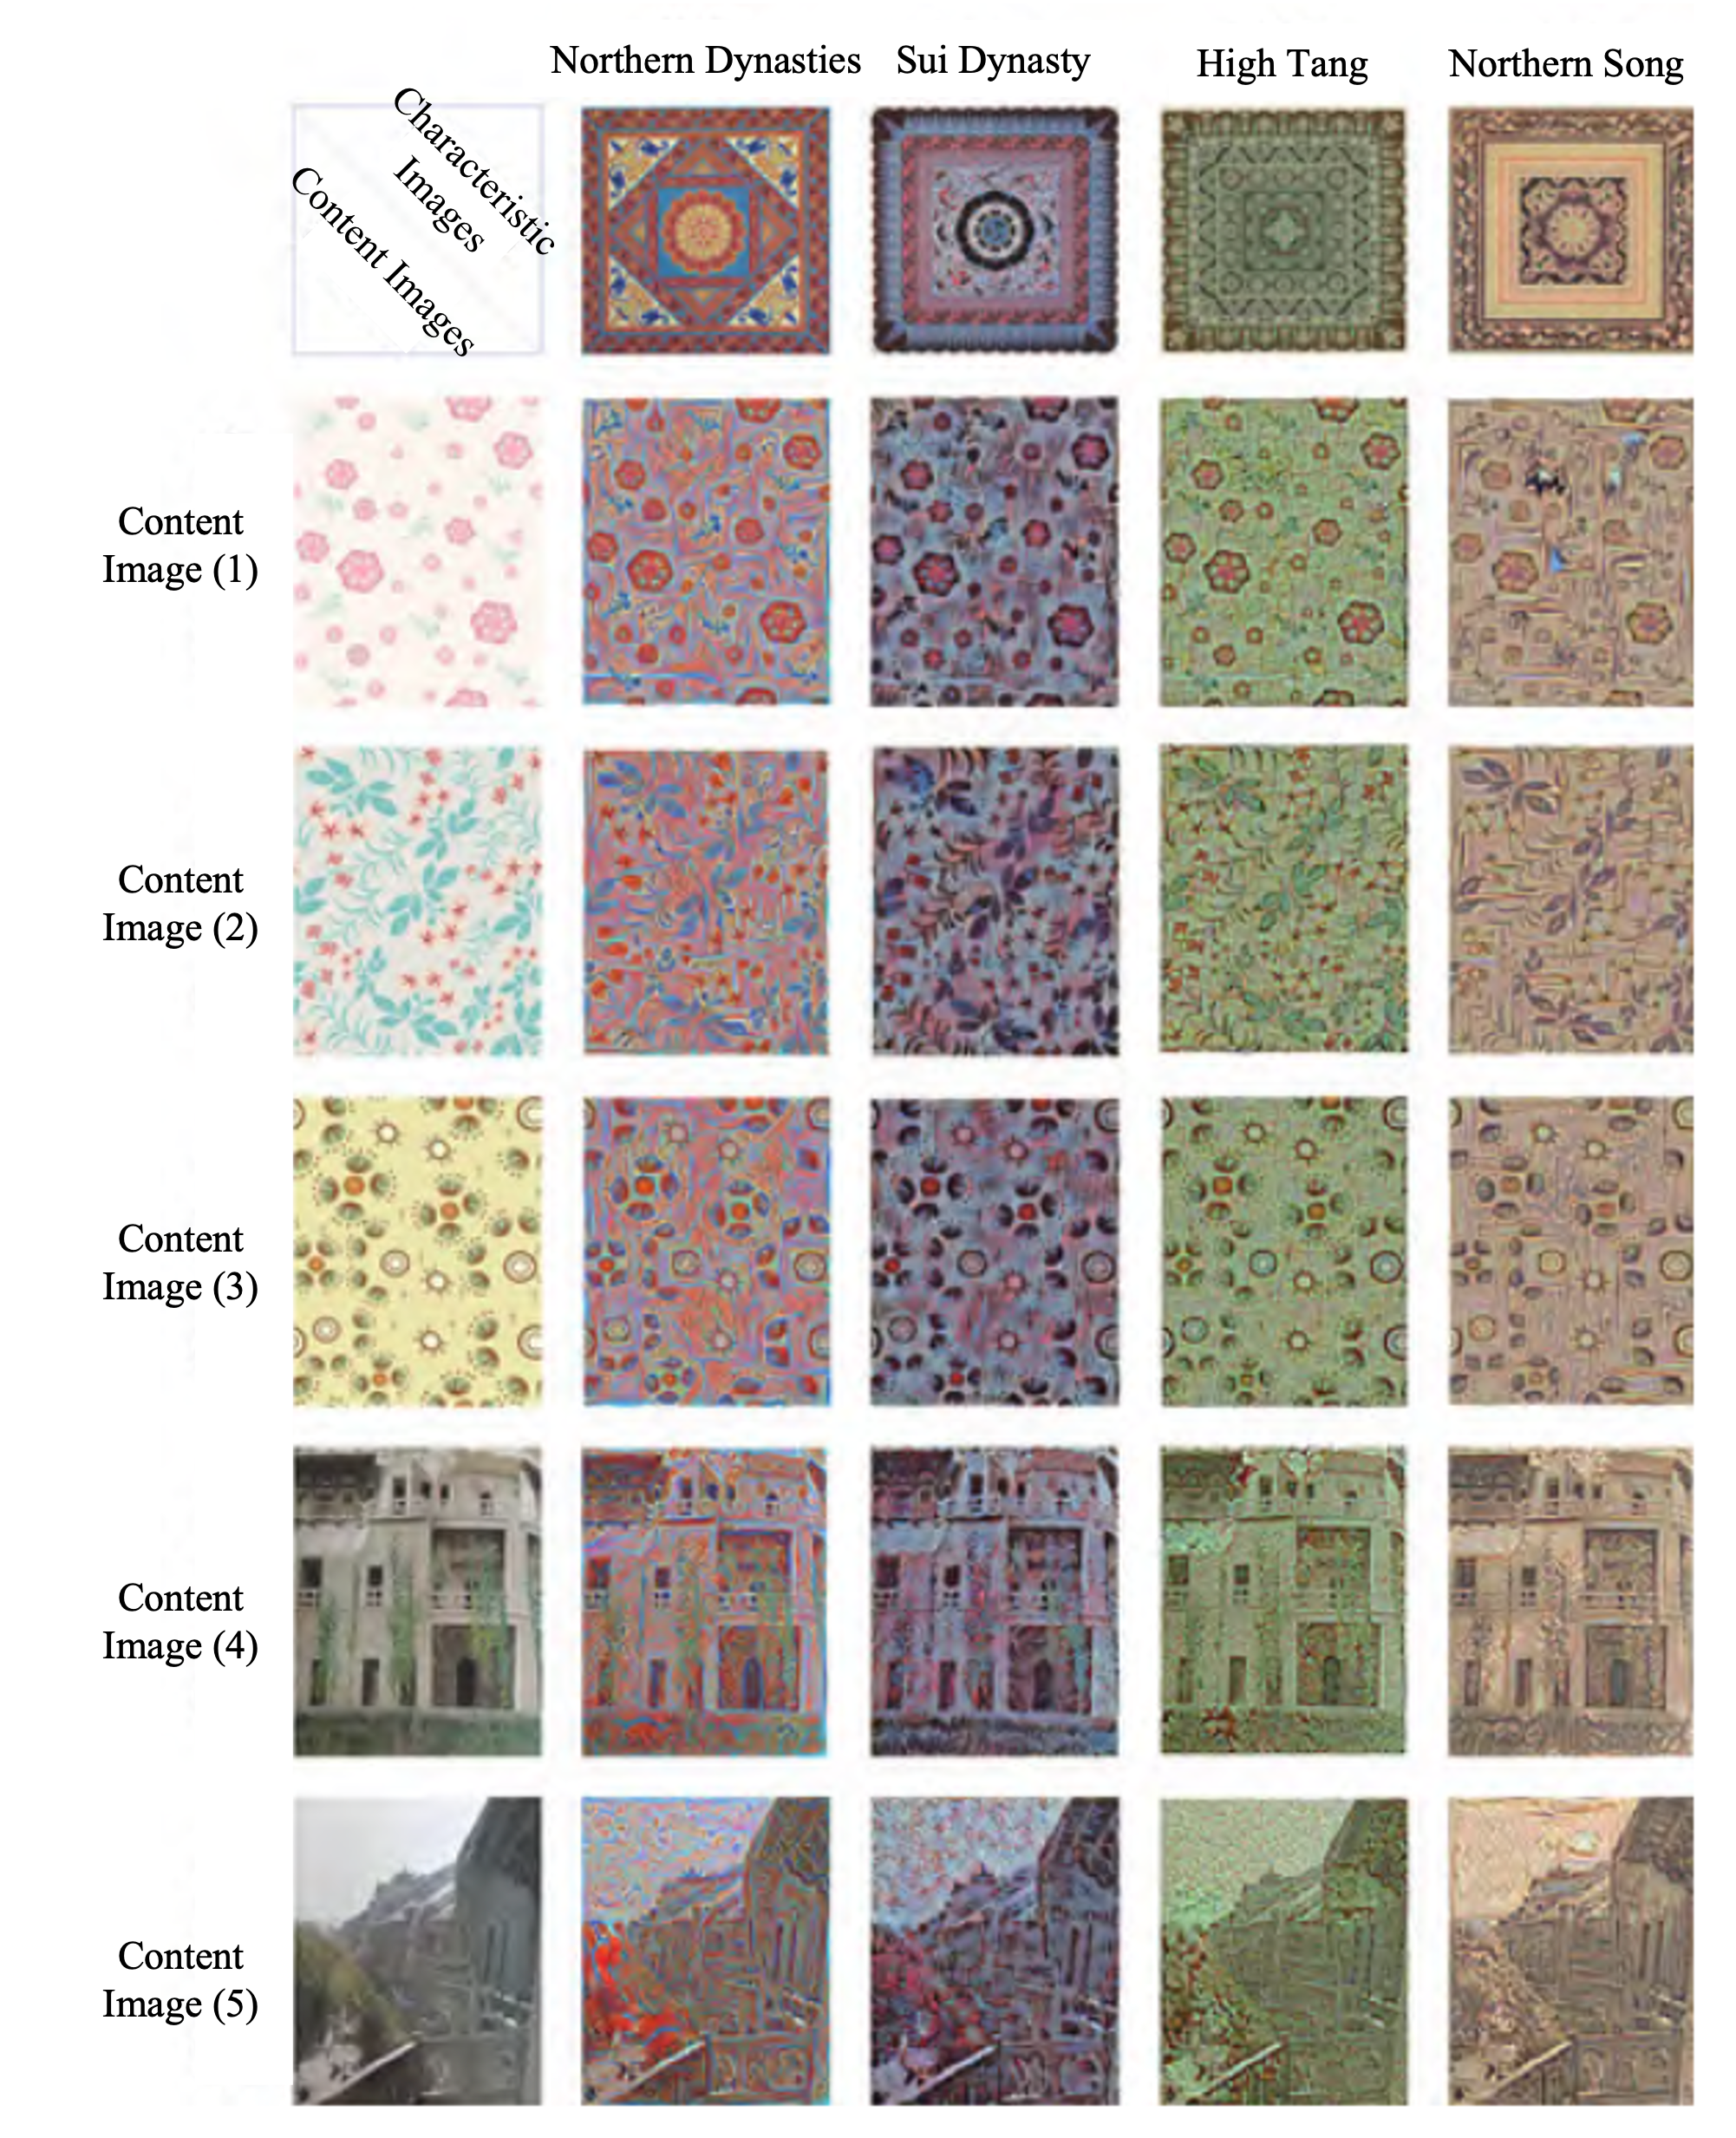
\includegraphics[width=0.9\textwidth]{figs/style-transfer-showcase-en.png}
    \end{center}

    \small\textit{Note.} The original figure were in Chinese. The captions are translted into English
    by the author. \apacitefigfrom{Sun2023-Dunhuang-Patterns}
\end{figure}

As deep learning and AI technologies rely heavily on large datasets, the demand of labelling imagery data,
especially for the research of Dunhuang Grottoes, is high (\apaciteaspar{Fu2025-AI-Intangible-Cultural-Heritage}).
Seeming to be paradoxical, the use of deep learning itself is the de facto solution for training deep learning
models for labelling images and objects automatically. \apaciteassub{Jiang2019-Deep-Learning-Object-Detection}
introduced some of the commonly used state-of-the-art models for object detection, including R-CNN and Fast R-CNN
(two-stage detectors), and You Only Look Once (YOLO) and Single Shot Detector (SSD) (one-stage detectors),
all of which are achieving satisfactory results in terms of accuracy and speed.
These models are now widely employed by renowned museums for archaeological research and preservation, such
as the Metropolitan Museum of Art (\apaciteaspar{Villaespesa2021-Computer-Vision-Metropolitan-Museum}),
Emperor Qin Shihuang's Mausoleum Site Museum (\apaciteaspar{Bevan2014-Computer-Vision-Archaeological-Classification}),
and, most importantly, the Dunhuang Research Academy (\apaciteaspar{Yu2022-AI-Dunhuang}).

\subsection{Natural Language Processing and Large Language Models}

Text-related technologies, such as NLP and LLMs, are predominantly used in both research and humanity aspects.
As these technologies are often used in collaboration with computer vision technologies, they are only briefly
introduced in this section.

In the archaeological research aspect, NLP technology is often used to transcribing and analysing the transcripts
of orally told history (\apaciteaspar{Fu2025-AI-Intangible-Cultural-Heritage}).
\apaciteassub{Fu2025-AI-Intangible-Cultural-Heritage} also mentioned the use of LLMs in generating documentations
for the artefacts, while \apasecciteassub{Manovich}{2017}{Fu2025-AI-Intangible-Cultural-Heritage} mentioned
providing commentaries for artefacts from innovative perspectives. In Dunhuang's case, the DHA has been leveraged
the capabilities of AI to recover and identify characters from excavated manuscripts from the Library Cave
(\apaciteaspar{Gansu2025-Digital-Library-Cave}).

In the humanity aspect, popular LLMs, such as ChatGPT, are used for interactive chatbots for public education
and addressing public enquiries (\apaciteaspar{DHAnd-Cave17-Smart-Library}; \apaciteaspar{Jiang2024-Digital-Dunhuang};
\apaciteaspar{Shen2024-LLM-History-Education}), and also smart search engines allowing users to look for specific
artefacts with natural language (\apaciteaspar{DHAnd-Cave17-Smart-Library}).

\section{AI Technologies Benefiting Buddhist Heritage Preservation}

\subsection{Automated Object Detection Accelerating Research}

The current advancements in computer vision and deep learning technologies plays a catalytic role in the research
of the Dunhuang Grottoes. As \apaciteassub{Resler2021-Deep-Learning-Archaeology} mentioned, the fundamental step
for researchers in the archaeological field is to fit the excavated artefacts into their appropriate categories
according to their features and attributes. It is not uncommon that this process relies heavily on the workers'
mastery of knowledge, personal preferences over certain styles (\apaciteaspar{Barcelo1995-Back-propagation};
\apaciteaspar{Yu2022-AI-Dunhuang}), and time dedicated to repetitive tasks.

Prior to the emergence of computer vision, the process of classification relied completely on researchers'
manual efforts. An experiment carried out by \apaciteassub{Verschoof2021-Automated-Object-Detection} studying
the integration of deep learning models in the classification of archaeological artefacts has shown that
the speed of work can be increased by 8 times. They also mentioned that the time of the researchers can be
reallocated to other steps in the analysis process, further enhancing the efficiency of the research.

In terms of applications in the preservation of Dunhuang Grottoes, the experiment by
\apaciteassub{Yu2022-AI-Dunhuang}, employing multiple models and analysis metrics, has given varied results
in terms of accuracy. The result showed that the YOLO v5-S model performed the best, with the
mean Average Precision (mAP\footnote{
    The mAP is a metric measuring the model's capabilities in correctly detecting and locating objects in images.
    The higher the value, the better the model's performance.
}) of 0.6809.

However, these methods are not without flaws. The performance of object detection models solely depends on the
dataset on which that they were trained, which implies that the number of already identified items directly
dictates the accuracy in identifying objects of the same kind. As \apaciteassub{Yu2022-AI-Dunhuang} pointed out,
there lacks a balance in the number of readily available labelled images of the artefacts in the e-Dunhuang
dataset, which may have resulted in the worst performance of the model when identifying non-Buddhist figures,
with accuracy of 0.6293 (while other categories reaching around 0.80).

To argue, it is important to recognise that the use of AI does not intend to subsitute the researchers, but rather
to act as a complementary tool to assist the current works
(\apaciteaspar{Verschoof2021-Automated-Object-Detection}). An ideal workflow would be to use the AI models for
a rough classification and tagging of the artefacts, and then to employ the researchers' intervention to further
sample and verify the results. While human intervention is still required, the efficiency of the research is indeed
enhanced. Therefore, it is reasonable to conclude that the use of computer vision and deep learning technologies
has high potential in accelerating the research of the Dunhuang artefacts, thereby benefiting the preservation
work.

\section{Concerns Raised Against AI Technologies in Buddhist Heritage Preservation}

\section{Conclusion}

\printbibliography